\documentclass[]{llncs}
%
\usepackage[english]{babel}
\usepackage{euscript}
\usepackage{mathrsfs,amssymb}
\usepackage{amsmath}
\usepackage{makeidx}
\usepackage{url}
\usepackage{color}
\usepackage{pslatex}
\usepackage{diffs}
\usepackage[latin1]{inputenc}
\usepackage[T1]{fontenc}
\usepackage{xspace}
\usepackage{subfigure}
\usepackage[pdftex]{graphicx}
\usepackage{comment}
\usepackage{tabularx}
\usepackage{soul}
\usepackage[page]{appendix}
\usepackage{subfigure}
\usepackage{enumerate}
\usepackage{enumitem}
\usepackage{moresize}
\usepackage{algpseudocode}
 

\usepackage{listings}

%% Kermeta Language
\definecolor{KRed}{rgb}{0.59,0,0}
\definecolor{KBlue}{rgb}{0,0,0.59}
\definecolor{KBlack}{rgb}{0,0,0}
\definecolor{KGreen}{rgb}{0,0.59,0}
\definecolor{KPurple}{rgb}{0.5,0,0.47}
\definecolor{KOliveGreen}{cmyk}{0.64,0,0.95,0.40}

\lstdefinelanguage{kermeta} { morekeywords=[0]{ require, using,
extern, pre, post, inv}, morekeywords=[1]{ package, inherits, class,
attribute, reference, property, readonly, getter, is, setter, alias,
enumeration, operation, method }, morekeywords=[2]{ aspect, abstract
}, morekeywords=[3]{ do, end, function, rescue, from, until, loop,
if, then, else, raise, var, init, raises }, morekeywords=[4]{ true,
false, void, result, value, self, super }, morekeywords=[5]{ bag,
set, seq, oset, Void}, morekeywords=[6]{ and, or, not },
sensitive=true, morecomment=[l]{//}, morecomment=[s]{/*}{*/},
morestring=[b]", }

\lstset{language=kermeta,
   basicstyle=\ttfamily,
   keywordstyle=[0]\bf\color{KRed},
   keywordstyle=[1]\bf\color{KBlue},
   keywordstyle=[2]\textit\bf\color{KBlue},
   keywordstyle=[3]\bf\color{KBlue},
   keywordstyle=[4]\textit\bf\color{KPurple},
   keywordstyle=[5]\bf\color{KBlack},
   keywordstyle=[6]\bf\color{KPurple},
   commentstyle=\color{KOliveGreen},
   tabsize=4,
   breaklines=true,
}

\newcommand{\noniso}{~\substack{\sqsubset\\ \sim}~}
\newcommand{\partialnoniso}[1]{~\substack{\sqsubset\\ \sim}_#1~}
\newcommand{\match}{\mbox{~<\#~}}
\newcommand{\deftitle}[1]{\emph{\textbf{(#1)}}}

\newcommand{\ie}{\emph{i.e.}, }
\newcommand{\eg}{\emph{e.g.}, }
\newcommand{\etal}{\emph{et al.} }

\declareuser{rf}{rf}{blue}
\declareuser{ps}{ps}{green}
\declareuser{bc}{bc}{magenta}

\begin{document}

\title{Using Model Types to Support \\Contract-Aware Model Substitutability}
\titlerunning{Using Model Types to Support Contract-Aware Model Substitutability}

\author{ %
	Wuliang Sun\inst{1}, Benoit Combemale\inst{2}, Steven Derrien\inst{2}, Robert B. France\inst{1}
}

\authorrunning{Sun et al.}

\institute{%
Colorado State University, Fort Collins, USA
\and
University of Rennes 1, IRISA, France
}

\maketitle
\thispagestyle{empty}

\setcounter{footnote}{0}

\begin{abstract}
	Model typing brings the benefit associated with well-defined type systems to model-driven development (MDD) through the assignment of specific types to models. 
In particular, model type systems enable reuse of model manipulation operations (e.g., model transformations), where manipulations defined for models typed by a supertype can be used to manipulate models typed by subtypes. 
Existing model typing approaches are limited to structural typing defined in terms of object-oriented metamodels (e.g., MOF), in which the only structural (well-formedness) constraints are those that can be expressed directly in metamodeling notations (e.g., multiplicity and element containment constraints).
In this paper we describe an extension to model typing that takes into consideration structural invariants, other than those that can be expressed directly in a metamodeling notation, and specifications of behaviors associated with model types. 
The approach supports contract-aware substitutability, where contracts are defined in terms of invariants and pre-/post-conditions expressed using OCL. 
Support for behavioral typing paves the way for behavioral substitutability.
We also describe a technique to rigorously reason about model type substitutability as supported by contracts, and apply the technique in a usage scenario from the optimizing compiler community.


\begin{comment}
Model typing extends the applicability of typing to model-oriented type
system by assigning models with specific types. It provides support for
model substitutability addressing a wide range of facilities such as model
transformation reuse. While existing approaches are limited to
object-oriented metamodels (e.g., MOF) as types, there is a need for
exploring more precise types. In particular, we propose in this paper an
extension to model typing that takes into account contract-aware
substitutability where contracts are defined in terms of invariants and
pre-/postconditions expressed using OCL. While invariants offer a suitable
way to complete object-oriented metamodels with additional structural
properties, pre-/postconditions pave the way of behavioral
substitutability for model transformation specialization. We also provide
an implementation to rigorously reason about the substitutability on model
types with contracts and apply it on use cases coming from the optimizing
compiler community.
\end{comment}
	
	\keywordname{SLE, Modeling Languages, Model Typing, Contract Matching, Model Substitutability}
\end{abstract}

\section{Introduction}

In Model Driven Engineering (MDE), developers of complex software systems create and transform models using model authoring and transformation technologies.
%Model transformations are used to facilitate interoperability among models expressed in different modeling languages.  
The rise in the number of new modeling languages, however, presents a challenge because it requires software engineers to create complex transformations that manipulate models expressed in the new languages. Building these transformations from scratch requires significant effort. To address this problem, various approaches \cite{Steel07}\cite{Varro04}\cite{Cuccuru07}\cite{Sanchez08}\cite{deLara10} have recently been proposed to facilitate the reuse of model transformation across different languages.  
%There is thus a need for MDE approaches that provide support for model transformation reuse.

Model substitutability rules that are based on model typing \cite{Steel07} can be used to support model transformation reuse.
%Model substitutability can be achieved through the subtyping relation between two model types.
For example, a subtyping relation that supports model substitutability allows a model typed by A to be safely used where a model typed by B is expected, where B is the supertype of A.
The transformation used for models typed by B can thus be reused on models typed by A.

Current approaches to model type definition and implementation, however, only consider MOF-based metamodels as model types. 
In MOF, contracts (e.g., pre-conditio-ns, post-conditions and invariants) are externally defined, that is, they are defined in another language, for example, the Object Constraint Language (OCL) \cite{OCL}. 
Neither the original paper on model typing \cite{Steel07} nor the follow-up paper \cite{ecmfa12} considers externally defined contracts in subtyping relations. This limits the utility of model subtyping in model-based software development approaches that  are contract based (e.g., design by contract \cite{meyer1992applying}).
There is thus a need for model typing that provides support for typing models with contracts.

In this paper we propose a form of model typing that supports contract-aware substitutability, where contracts are defined in terms of invariants and pre-/post-conditions expressed using OCL. 
We add invariants to model types that specify additional structural properties, and use operation pre-/post-conditions to specify the transformation rules on model types. 
We also describe a technique for rigorously reasoning about the substitutability of models with contracts.
 
The rest of the paper is organized as follows. 
Section \ref{examples} illustrates the need for contract-aware substitutability using motivating examples from the high-performance 
embedded system design domain.
Section \ref{background} presents background material needed to understand the work described in this paper.
Section \ref{contribution} presents a formal definition  of the subtyping relation between two model types that include contracts, 
and describes tool support for reasoning about substitutability on model types.
Section \ref{discussion} describes limitations of the approach.
Section \ref{relatedwork} discusses related work, and Section \ref{conclusion} concludes the paper with a discussion of planned future work. 
%The interest to make contract-aware the class matching algorithm is twofold:
%- invariants: in the definition/checking of the subtyping relation. Until now, the subtyping relation was defined between 2 MOF metamodels. This relation will now be defined between 2 MOF+OCL metamodels (considering now the Well Formedness Rules in the metamodel, in addition to the object-oriented structure provided by the MOF classes and references).
%- pre-/post-conditions: in the checking of the subtyping relation. The consideration of the pre- and post-conditions will make possible the redefinition (and not only the reuse) of operation (i.e., model transformation in our case), being able to check the behavioral substitutability based on an axiomatic specification of what the operation do. Transformation rules pave the way of behavioral substitutability for model transformation specialization.

%\input{introduction_old20130214.tex}

\section{Motivating Examples}\label{examples}

In this section we describe two motivating examples from the high-performance embedded system design domain. 
Modern heterogeneous embedded hardware platforms are notoriously difficult to design and to program. 
In this context, tool-supported model based approaches (e.g., Simulink, Ptolemy) are now widely acknowledged as some of the most 
effective approaches to designing embedded systems. 

Typically, these model-based approaches use tool chains that manipulate many different types of models. 
For example, structural platform description models range from system level models that abstract over processing and storage resource with their interconnections, to very low level Register-to-Logic level circuit models that are used to describe the structure of hardware accelerators within the platforms.

Similarly, behavioral description models range from application level modeling of the 
application using Models of Computation such as Synchronous Data Flow Graphs or 
Kahn Process Networks, to fine grain scalar operation level representations such as the 
basic-block level instruction dependence graph used in an optimizing compiler back-end. 

Most of these tool chains share a common goal: They aim to produce highly optimized  
implementations. This requires the use of advanced algorithms that implement very complex model manipulations. 
It is also the case that these manipulations often have similar algorithmic patterns. These patterns can be used as the basis for
developing reusable model transformations.


\subsection{Example 1: Using Model Types to Support Structural Substitutability}\label{structuralexample}

In the optimizing compiler domain, a variety of models describing different aspects of languages are manipulated (i.e., analyzed and transformed) at different stages of the compilation process. While the analyses and transformations are different, they also share many common characteristics.
For example, consider algorithms for schedule optimization. 
Obtaining an optimized implementation of an application on a target platform 
involves performing several static scheduling optimizations. 
Many of these algorithms have common characteristics, for example, they are often expressed as an acyclic graph resource constrained scheduling problem, for which many 
techniques (heuristics or MILP-Mixed Integer Linear Programming-solver based) have been proposed. 
Because these scheduling algorithms involve very sophisticated algorithms, reusable algorithms that can be tailored to the different types of representations (models) are highly desirable. 
For example, it would be useful to have a reusable scheduling algorithm that can be used to derive a schedule for an Application level Synchronous Data-flow graph on a multi-processor 
based implementation, as well as for generating efficient code for a customized VLIW (Very Long Instruction Word) embedded 
processor.        

However in this case, structural substitutability based only on constraints that can be expressed directly in a metamodel (e.g.,  multiplicity or element containment constraint) is not sufficient; other structural constraints need to be specified. 
For example, a classical static scheduling toolset can only operate on acyclic dependence graphs and the 
acyclicity property cannot be expressed directly in a metamodel. 
A language such as the Object Constraint Language (OCL) is needed to specify properties of acyclic graphs. 
In this case, model substitutability requires that a substitute model enforces the acyclicity constraint expressed in OCL.      
Model typing based on metamodels with OCL constraints can be used to enable such structural substitutability.

\subsection{Example 2: Using Model Types to Support Contract-based Behavioral Substitutability}\label{behavioralexample}

\subsubsection*{Behavioral substitutability for model transformations:}

A consistent scheduling tran-sformation must ensure that every node in the dependence graph is scheduled 
\emph{at least} once. This property can be expressed as a post-condition on the scheduling transformation and thus any scheduler 
implementation should enforce this post-condition. The effective post-condition could even be 
stricter; in our case we could consider a post-condition that restricts a node to be scheduled 
\emph{exactly} once.

% TODO steven : Figure for scheduling+mapping plus codegeb. 

The same holds for the pre-condition. For example, most schedulers operate on acyclic graphs and this can 
be translated as a pre-condition for the transformation. However, there also exists a class of 
pipelined schedulers that operate on cyclic graphs, in which cycles implement delays to preserve 
causality. For such pipelined schedulers, the pre-condition would not forbid cycles in the dependence graph.
That would, however, prevent a pipelined scheduler from being used to schedule 
acyclic graphs in a design flow.    

\subsubsection*{Contract based tool chain validation:}

An optimizing compiler custom tool chain consists of a sequence of analyses and transformations (called 
compiler passes) executed in a very carefully chosen order. They can hence be seen as a model 
transformation chain. Compiler passes cannot be combined arbitrarily, as each pass 
usually assumes that the program representation at hand has very specific properties.    

\begin{figure}[!t]
\centering
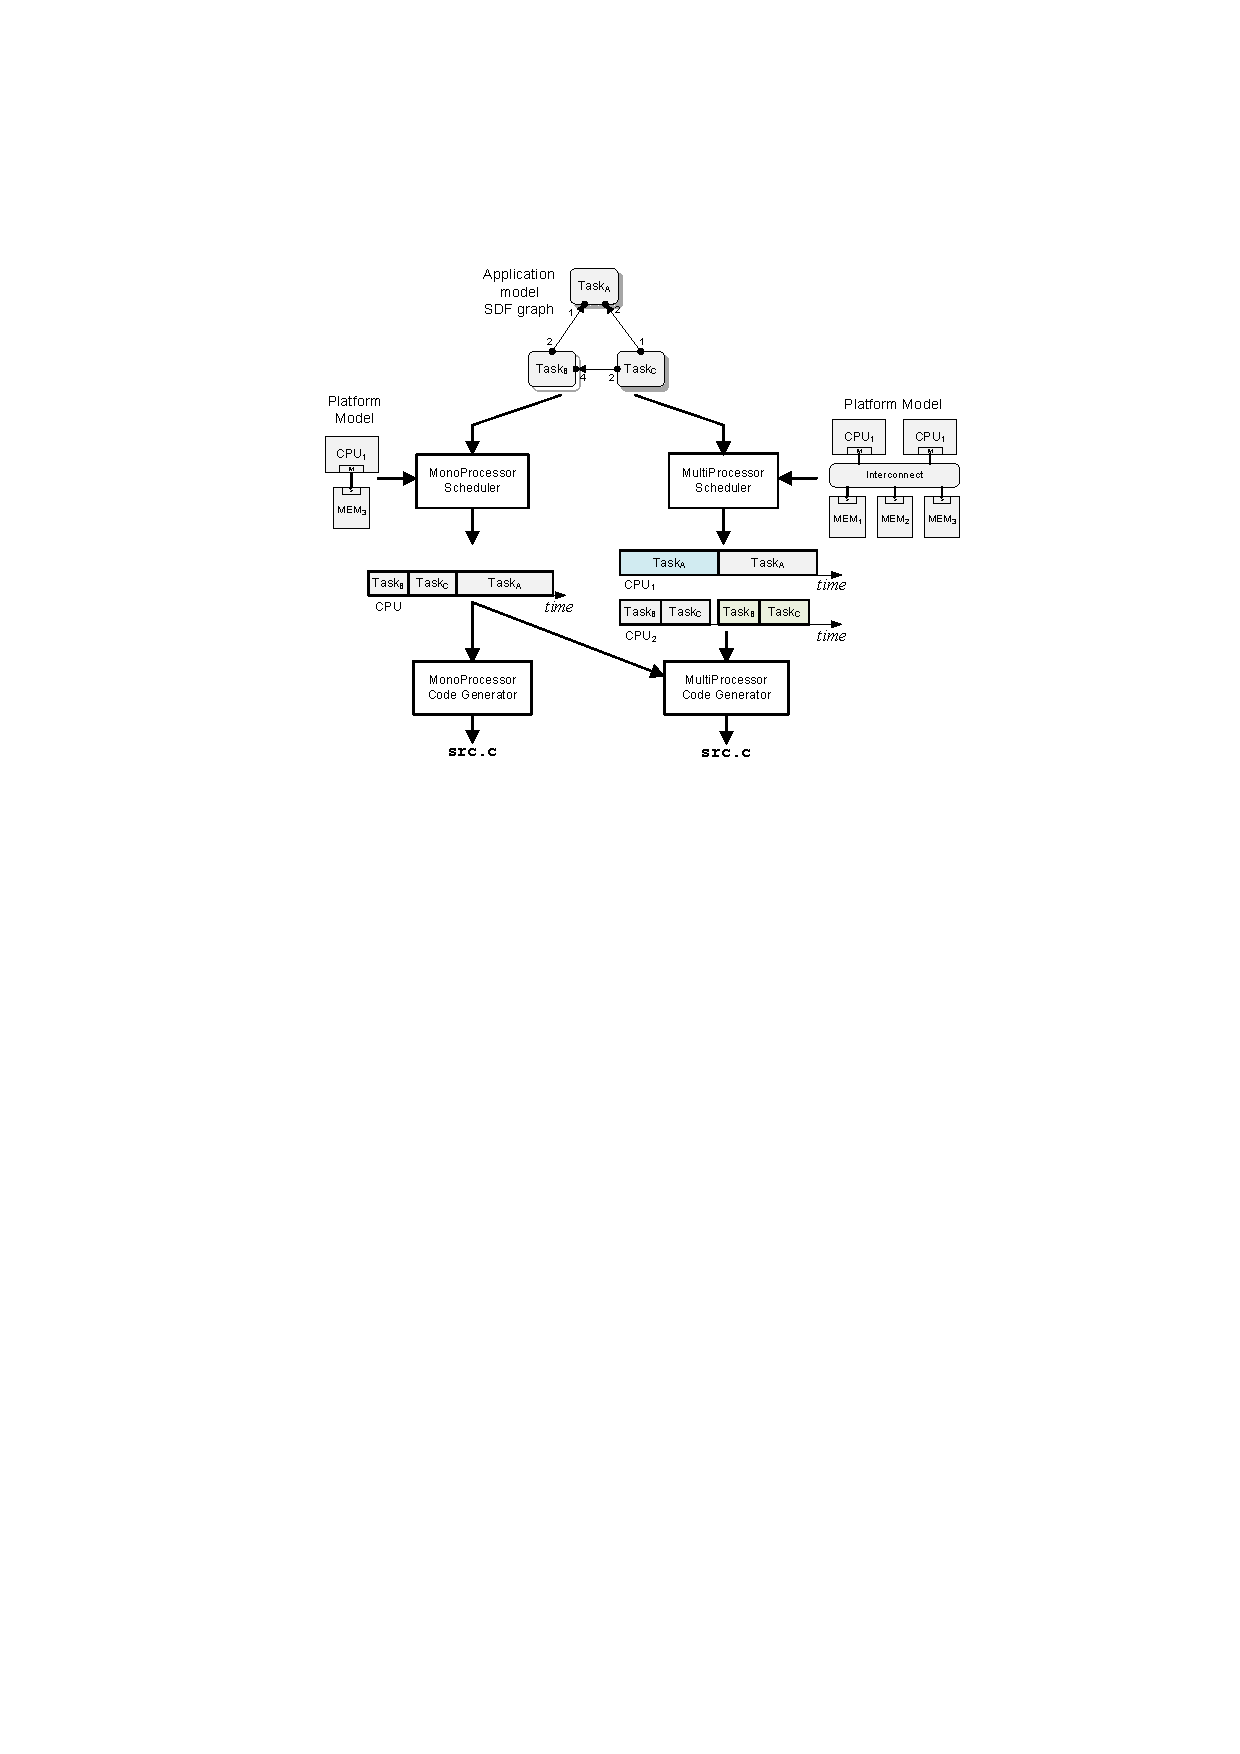
\includegraphics[width=4in]{fig/SDF-flow.pdf}
\caption{A Model based compiler tool chain for embedded multiprocessors. 
%The toolchain is used to   
%schedule a synchronous dataflow task graph on either a single or multi-processor depending 
%on the chosen scheduling component and platform model. Two back-end code generators are 
%provided. The monoprocessor code generator can only be used after a uniprocessor 
%scheduling stage, whereas the second back-end is more general and can be used for 
%both type of scheduling.     
}
\label{fig:toolchain}
\end{figure}


For example, consider a compiler tool chain for generating software code from 
Synchronous Data Flow Graph (SDF) model specifications on an embedded
platform. Such a tool chain is illustrated in Figure~\ref{fig:toolchain}.
Before any code can be produced, the SDF first needs to be scheduled on
this platform. Depending on whether the target system consists of a single or
several processors, it is likely that different scheduling algorithms will be
used. Similarly, different code generators (i.e. pretty printers) will have to
be used depending on whether we target a mono-processor or multiprocessor. Two back-end code generators are 
shown in Figure~\ref{fig:toolchain}. The mono-processor code generator can only be used after a mono-processor 
scheduling stage, whereas the second back-end is more general and can be used for 
both types of scheduling.     

These constraints -- that is targeting one or several processing resources --
apply to the result of the scheduling stage and to the input on the code
generation stage. They can hence be modeled as pre-conditions (resp.
post-conditions) expressed using OCL. When chaining a given scheduling and
code generation pass, we can ensure the consistency of the flow by checking if
the pre-/post-conditions of two chained transformation are satisfiable.



  
%\input{examples_old20130214.tex}

%\section{Background: On Model Typing} 
%
%- Model Typing to achieve substitutability, 
%- subtyping relation, 
%- class matching relation
%==> limitation : the class matching relation is not taken into account of the matching of the contracts.
%	
%%%%%%

\section{Background}\label{background}

In this section, we describe the concepts underlying our use of model types to support model substitutability.
%Model typing provides a well-defined theory that considers models as first-class entities, and typed by their respective model types~\cite{Steel07}, where model substitutability is achieved through subtyping relations between model types.  These relations enable a model typed by $A$ to be safely used where a model typed by $B$ is expected, $A$ and $B$ being model types.
We first present the MOF (Meta-Object Facility) meta-language, the basis for metamodels, and thus model manipulation operators. We then give an overview of model types as currently defined and implemented \cite{Steel07,ecmfa12}, and describe the limitations addressed by the approach presented in this paper. 

\subsection{Metamodeling}

{\em The Meta-Object Facility} (MOF)~\cite{MOF} is the OMG's standardized meta-language, i.e., a language to define metamodels. As such, it is a common basis for a vast majority of modeling languages and tools. A metamodel defines a set of models on which it is possible to apply common operators. The model substitutability approach presented in this paper is applicable to models expressed in languages with MOF metamodels. 

%\begin{figure}[tb]
%	\center
%	\includegraphics[scale=0.6]{fig/MOF.pdf}
%	\caption{The EMOF core with class diagram notation}
%	\label{MOF}
%\end{figure}

%Figure~\ref{MOF} displays the structure of EMOF (Essential MOF) which contains the core of the MOF meta-language in the form of a class diagram. E
MOF supports the definition of metamodels using \texttt{Classes} and \texttt{Properties}.\\ \texttt{Classes} can be abstract (i.e., they cannot be instantiated) and have \texttt{Properties} and \texttt{Operations}, which respectively declare attributes and references, and the signatures of methods available to the modeled concept. 
%\texttt{Classes} can have several super classes, from which they inherit all \texttt{Properties} and \texttt{Operations}.
A \texttt{Property} can be composite (an object can only be referenced through one composite \texttt{Property} at a given instant), derived (i.e., calculated from other \texttt{Properties}) and read-only (i.e., cannot be modified). A \texttt{Property} can also have an opposite \texttt{Property} with which it forms a bidirectional association.
%An \texttt{Operation} declares the \texttt{Types} of the exceptions it can raise and ordered \texttt{Parameters}.
%\texttt{Propertys}, \texttt{Operations}, and \texttt{Parameters} are \texttt{TypedElements}; their type can be either: a \texttt{Datatype} (\eg \texttt{Boolean}, \texttt{String}, etc.) or a \texttt{Class}.
%\texttt{Parameters}, \texttt{Properties} and \texttt{Operations} are \texttt{Multiplicity Elements}. As such, they have a multiplicity (defined by a lower and an upper bound), as well as orderedness and uniqueness.


{\em Metamodels} can be viewed as class diagrams in which each metamodel element can be instantiated to obtain objects representing model elements. However, metamodel elements are themeslves instances of MOF elements and thus a metamodel can be drawn as an object diagram where each concept is an instance of one of the MOF elements (e.g., \texttt{Class} or \texttt{Property} classes).

%Because model subtyping takes place at the metamodel level, the latter representation facilitates the definition of model subtyping relations by depicting metamodels and their contained concepts as objects with attributes and properties. 
%Thus, we will use the object diagram representation in preference to the more common class diagram one.

\subsection{Model Typing}\label{modeltyping}

{\em Model Types} were introduced by Steel \etal \cite{Steel07}, as an extension of object typing to provide abstractions about the object type level and enable the reuse of model manipulation operators.  Informally, a model type is a substructure (referred to as a {\em type group}) of the metamodel's class diagram.  It is important to distinguish the usage of the term metamodel from model type. We use the term metamodel to refer to the class diagram used to define a language, and when the same class diagram is used to define the type of a model it is called an {\em exact type}. It is also important to note that a model has one and only one metamodel to which it must conform, but the same model can have several model types, where each model type is a substructure of the metamodel. Because model types and metamodels share the same structure, it is possible to extract the exact type of a model from its metamodel. Figure~\ref{3lvl} represents a model $m_1$ that conforms to a metamodel $MM_1$ and is typed by model types $MT_A$ and $MT_B$, where $MT_B$ is the \emph{exact type} of $m_1$ that is extracted from $MM_1$. Both metamodels and model types conform to MOF.
\begin{figure}[tb]
	\center
	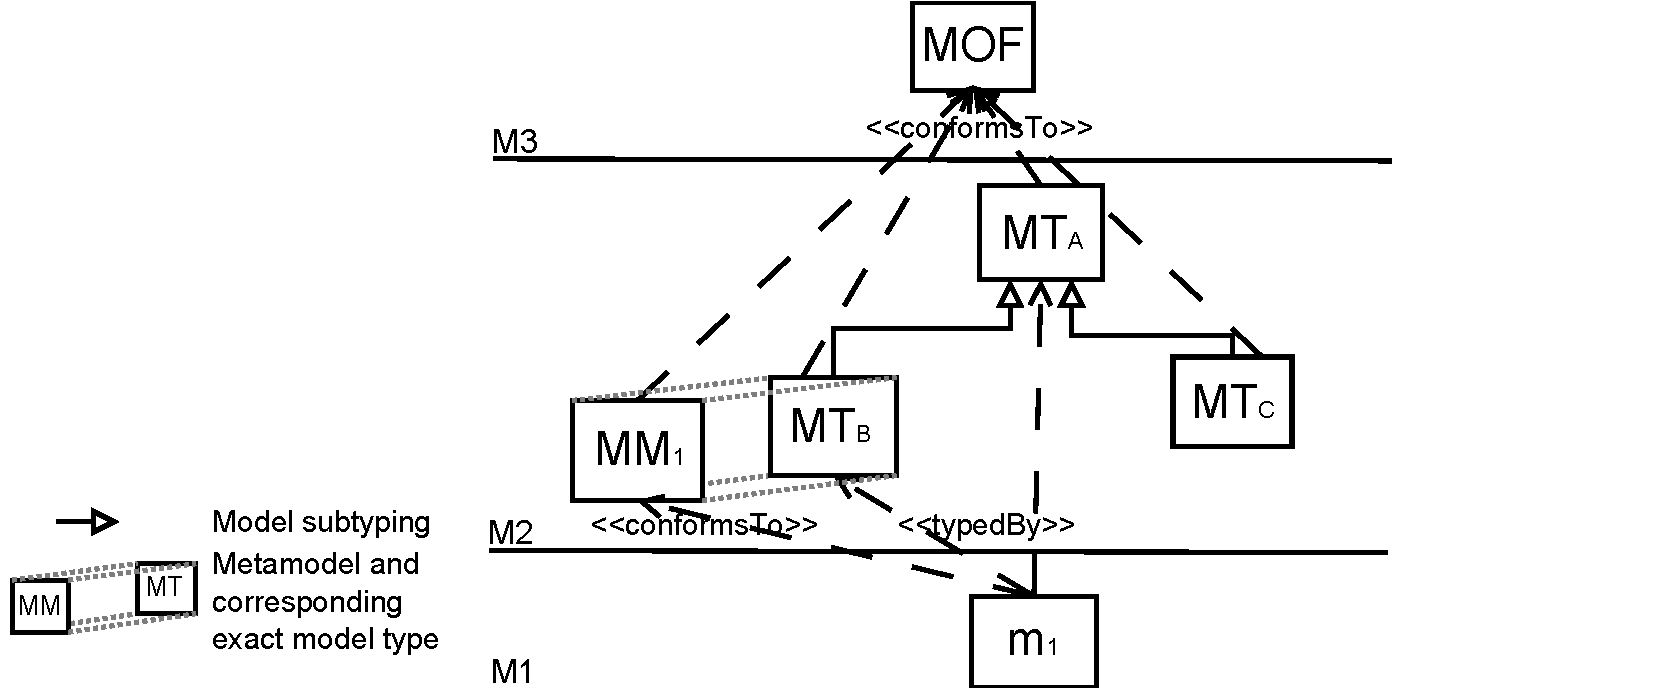
\includegraphics[scale=0.37]{fig/3levels2.pdf}
	\caption{Conformance, model typing and model subtyping relations}
	\label{3lvl}
\end{figure}
Given the above, a model type can be defined as follows:
\begin{definition}\label{modeltypedef}
\deftitle{Model type}
A model type is a substructure of a metamodel's class structure. A model does not have to include instantiations of each class in an associated model type, that is, the set of classes of elements in a model can be smaller than the classes in its model type.
\end{definition}

{\em Substitutability} is the ability to safely use an object of type $A$ where an object of type $B$ is expected. 
Substitutability is supported through subtyping in object-oriented languages. However, object subtyping does not handle specializations of model substructures (or {\em type groups})\footnote{For further information on type groups see Ernst's paper~\cite{Ernst01}.}. 
%Such type group specialization have been explored by K\"{u}hne in the context of MDE~\cite{Kuhne12}. K\"{u}hne defines three model specialization relations (specification import, conceptual containment and subtyping) implying different level of compatibility. We are only interested here in the third one, subtyping, which requires an \emph{uncompromised mutator forward-compatibility}, \eg substitutability, between instances of model types.
%\subsubsection{MOF Class Matching}
One way to safely reuse a model manipulation operation created for a model typed by $MT_A$ on a model typed by $MT_B$ is to ensure that $MT_A$ contains elements that can be substituted by elements defined by $MT_B$. 
%Since only model types conforming to MOF are currently considered, this can be done by ensuring the MOF elements from $MT_B$ (\eg classes, properties, operations) substitutable for those contained by $MT_A$. 
However, it is not possible to achieve model type substitutability through object subtyping. Thus, model typing uses an extended definition of \emph{object type matching} introduced by Bruce \etal \cite{Bruce03}, namely \emph{MOF Class Matching}.

\begin{definition}
\deftitle{MOF class matching}
MOF class $T'$ matches $T$ (written $T' \match T$) iff their names are equal, and for each property (respectively method) in $T$ there is a corresponding property (respectively method) in $T'$.
\end{definition}

The \emph{MOF class matching} relation can be seen as a kind of \emph{object type matching} relation that is tailored to MOF concepts.
Based on the \emph{MOF class matching} relation, we can achieve model type substitutability by defining a subtyping relation as follows:

\begin{definition}
\deftitle{Subtyping relationship for model types}
The model type \emph{subtyping} relation is a binary relation $\sqsubseteq$ on $ModelType$, the set of all model types, such that $(MT_B, MT_A) \in \sqsubseteq$ (also written $MT_B \sqsubseteq MT_A$) iff  $\forall$ $T_A$ $\in$ $MT_A$, $\exists$ $T_B$ $\in$ $MT_B$ such that $T_B$ $\match$ $T_A$.
\end{definition}

We recently introduced four extended subtyping relations between model types that take into account two additional criteria: The presence of heterogeneities between two model types (using adaptation) and the considered subset of the model types (using model type pruning) \cite{ecmfa12}.

%\subsubsection{Limits of Model Subtyping}
The \emph{subtyping} relation as currently defined has shortcomings. 
In particular, the current model typing definition and implementation only considers MOF-based metamodels as model types (through the \emph{MOF class matching} relation). Unfortunately, MOF delegates the definitions of contracts (\eg pre and post-conditions or invariants) to other languages (\eg OCL, the Object Constraint Language~\cite{OCL}). 
%Hence neither the original paper on model typing~\cite{Steel07} nor the follow-up \cite{ecmfa12} considers contracts in subtyping relations, but focuses on features of object types contained by model types. 
This limits the applicability of model typing for safely reusing model manipulations where OCL contracts are needed to precisely specify the applicability of the model transformation or the structure on which the model transformation can be applied (see motivating examples in Section \ref{examples}). The approach described in this paper addresses this limitation.

%\input{background_old20130214.tex}

\section{Contribution}\label{contribution}

%The previous work on model typing \cite{ecmfa12} introduces substitutability into model types, and formally defines a subtyping relation between two model types specified using MOF\cite{MOF}.
%The previous work, however, only considers MOF-based structural subtyping in which the structure of two model types determines whether one is subtype of the other, which limits the applicability of model subtyping in a setting where OCL contracts are needed to precisely define modeling languages (e.g., specifying a model transformation).

In this paper we extend the subtyping relation described in \cite{ecmfa12} by taking into account OCL contracts for a safe substitutability of models conforming to metamodels including contracts. This provides a safe reuse of model transformations expressed on metamodels that include contracts. 
Specifically, we extend the MOF class matching (cf. Def. 2 of Section \ref{background}) by considering contracts matching (Section \ref{classmatching}) and provide a technique for analyzing the matching of OCL contracts associated with two classes with different model types (Section \ref{analyzingcontract}). In this section we describe the contract matching technique we developed to support contract-aware model substitutability. We also describe an Alloy-based prototype tool that supports contract matching (Section \ref{toolsupport}), and illustrate the use of contract-aware substitutability using the motivating examples (Section \ref{casestudy}).    

\subsection{Contract-aware MOF Class Matching}\label{classmatching}

We consider the use of OCL invariants added to MOF classes to specify additional structural properties, and OCL pre-/post-conditions defined in the context of MOF class operations to specify the model manipulation rules (e.g., transformation) associated with model types. 
The MOF class matching relation is thus determined by two aspects: the structural features specified using MOF (e.g., classes, properties, operation signatures, etc.) and the contracts expressed using OCL (e.g., invariants and pre-/post-conditions).  
%While the previous work \cite{ecmfa12} used the structural elements (cf. Def. 3 of \cite{ecmfa12}) to determine the matching relation between two MOF classes, the focus of this paper is to provide a formal definition of the contract matching used to support the contract-aware MOF class matching.  

The substitutability through model subtyping is a specialization of the Liskov Substitution Principle \cite{liskov1994behavioral} on the model type system. 
Specifically the contract matching relation that enables contract-aware model substitutability must abide by the following rules: (1) invariants of the supermodel type cannot be weakened in a sub model type, (2) pre-conditions cannot be strengthened in a sub model type, and (3) post-conditions cannot be weakened in a sub model type.
The extended MOF class matching relation is formalized as follows:

\begin{definition}[Contract-aware MOF Class Matching] Class $T'$ matches T (written $T'$ <\# T) iff their structures match (cf. Def. 3 of \cite{ecmfa12}), their invariants match and their operation pre-/post-conditions match, where
\begin{enumerate}
\item[1] \textbf{Invariants Match} is defined as follows:\\
let T.ownedInvariant = $\{$$inv_{T1}$, $inv_{T2}$, ..., $inv_{Tk}$ $\}$ be the invariants defined for $T$;\\
let $result_T$ = $inv_{T1}$ $\wedge$ $inv_{T2}$ $\wedge$ ... $\wedge$ $inv_{Tk}$;\\
let SuperClass(T) = $\{$$cls_1$, $cls_2$, ..., $cls_n$$\}$ where $cls_i$ is a superclass of T; \\
let $cls_i$.ownedInvariant = $\{$ $inv_{i1}$, $inv_{i2}$, ..., $inv_{ik}$ $\}$ be the invariants defined for $cls_i$, for i = 1, .., n;\\
let $result_i$ = $inv_{i1}$ $\wedge$ $inv_{i2}$ $\wedge$ ... $\wedge$ $inv_{ik}$, for i = 1, .., n;\\
let invs = $result_1$ $\wedge$ $result_2$ $\wedge$ ... $\wedge$ $result_n$ $\wedge$ $result_T$;\\
\\
let T$'$.ownedInvariant = $\{$$inv'_{T1}$, $inv'_{T2}$, ..., $inv'_{Tk}$ $\}$ be the invariants defined for $T'$;\\
let $result'_T$ = $inv'_{T1}$ $\wedge$ $inv'_{T2}$ $\wedge$ ... $\wedge$ $inv'_{Tk}$;\\
let SuperClass(T$'$) = $\{$$cls'_1$, $cls'_2$, ..., $cls'_n$$\}$ where $cls'_i$ is a superclass of T$'$; \\
let $cls'_i$.ownedInvariant = $\{$ $inv'_{i1}$, $inv'_{i2}$, ... , $inv'_{ik}$ $\}$ be the invariants defined for $cls'_i$, for i = 1, .., n;\\
let $result'_i$ = $inv'_{i1}$ $\wedge$ $inv'_{i2}$ $\wedge$ ... $\wedge$ $inv'_{ik}$, for i = 1, .., n;\\
let invs$'$ = $result'_1$ $\wedge$ $result'_2$ $\wedge$ ... $\wedge$ $result'_n$ $\wedge$ $result'_T$;\\
\\
The invariants of T and T$'$ match if Models(invs) $\supseteq$ Models(invs$'$), where $Models(invs)$ returns all models that satisfy $invs$ and $Models(invs')$ returns all models that satisfy $invs'$.\\
%\begin{algorithmic}
%\State let result1 = true, result2 = true, invs = true, invs$'$ = true
%\For {each cls in SuperClass(T)}
%    \For {each inv in cls.ownedInvariant} 
%		 		\State {result1 = result1 $\wedge$ inv}
%    \EndFor 
%    \State {invs = invs $\wedge$ result1}
%\EndFor 
%\For {each cls$'$ in SuperClass(T$'$)}
%    \For {each inv$'$ in cls$'$.ownedInvariant} 
%		 		\State {result2 = result2 $\wedge$ inv$'$}
%    \EndFor 
%    \State {invs$'$ = invs$'$ $\wedge$ result2}
%\EndFor 

%\State Models(invs) $\supseteq$ Models(invs$'$)
%\end{algorithmic}

%let invs: Constraint = SuperClasses(T)$\rightarrow$iterate(cls: Class, result1 : Constraint = true $|$ result1 and cls.ownedInvariant$\rightarrow$iterate(inv: Constraint, result2 : Constraint = true$|$ result2 and inv)),\\ 
%let invs$'$: Constraint = SuperClasses(T$'$)$\rightarrow$iterate(cls: Class, result1 : Constraint = true$|$ result1 and  cls.ownedInvariant$\rightarrow$iterate(inv: Constraint, result2 : Constraint = true $|$ result2 and inv)),\\
%invs $\supseteq$ invs$'$\\

%{\em Note that {\em SuperClasses(T)} returns $T$ plus all super classes of $T$.
%$invs$ is the conjunction of the invariants defined in the context of $T$ and its super classes, and $invs'$ is the conjunction of the invariants defined in the context of $T'$ and its super classes.
%{\em Models(invs)} returns all models that satisfy $invs$. 
%The clause {\em Models(invs) $\supseteq$ Models(invs$'$)} specifies that the models satisfying $invs$ must include the models satisfying $invs'$ (i.e., $invs$ are weaker than $invs'$).}\\
 
\item[2] \textbf{Pre-/post-conditions Match} is defined as follows:\\
$\forall$ op $\in$ T.ownedOperation, $\exists$ $S'$ $\in$ SuperClasses($T'$) such that $\exists$ $op'$ $\in$ $S'$.ownedOperation and:\\
	\begin{enumerate}
		\item[2.1] 
		let op.ownedPrecondition = $\{$$pre_{1}$, $pre_{2}$, ..., $pre_{k}$ $\}$ be the pre-conditions defined for $op$;\\
		let pres = $pre_{1}$ $\wedge$ $pre_{2}$ $\wedge$ ... $\wedge$ $pre_{k}$;\\
		let op$'$.ownedPrecondition = $\{$$pre'_{1}$, $pre'_{2}$, ..., $pre'_{k}$ $\}$ be the pre-conditions defined for $op'$;\\
		let pres$'$ = $pre'_{1}$ $\wedge$ $pre'_{2}$ $\wedge$ ... $\wedge$ $pre'_{k}$;\\
		\\
		%\begin{algorithmic}
		%	\State let pres = true, pres$'$ = true,
		%	\For {each pre in op.ownedPrecondition}
		%		\State {pres = pres $\wedge$ pre}
		%	\EndFor
		%	\For {each pre$'$ in op$'$.ownedPrecondition}
		%		\State {pres$'$ = pres$'$ $\wedge$ pre$'$}
		%	\EndFor
		%	\State Models(pres$'$) $\supseteq$ Models(pres)
		%\end{algorithmic}
		
		
		%let pres$'$: Constraint = op$'$.ownedPrecondition$\rightarrow$iterate(pre: Constraint, result : Constraint = true $|$ result and pre), \\
		%let pres : Constraint = op.ownedPrecondition$\rightarrow$iterate(pre: Constraint, result : Constraint = true $|$ result and pre), \\
		%pres$'$ $\supseteq$ pres
		\item[2.2] 
		let op.ownedPostcondition = $\{$$post_{1}$, $post_{2}$, ..., $post_{k}$ $\}$ be the post-conditions defined for $op$;\\
		let posts = $post_{1}$ $\wedge$ $post_{2}$ $\wedge$ ... $\wedge$ $post_{k}$;\\
		let op$'$.ownedPostcondition = $\{$$post'_{1}$, $post'_{2}$, ..., $post'_{k}$ $\}$ be the post-conditions defined for $op'$;\\
		let posts$'$ = $post'_{1}$ $\wedge$ $post'_{2}$ $\wedge$ ... $\wedge$ $post'_{k}$;\\
		\\
		The operation specifications of T and T$'$ match if Models(pres$'$) $\supseteq$ Models(pres) and Models(posts) $\supseteq$ Models(posts$'$)
		%\begin{algorithmic}
		%	\State let posts = true, posts$'$ = true,
		%	\For {each post in op.ownedPostcondition}
		%		\State {posts = posts $\wedge$ post}
		%	\EndFor
		%	\For {each post$'$ in op$'$.ownedPostcondition}
		%		\State {posts$'$ = posts$'$ $\wedge$ post$'$}
		%	\EndFor
		%	\State Models(posts) $\supseteq$ Models(posts$'$)
		%\end{algorithmic}
		
		%let posts$'$: Constraint = op$'$.ownedPostcondition$\rightarrow$iterate(post: Constraint, result : Constraint = true $|$ result and post),\\
		%let posts : Constraint = op.ownedPostcondition$\rightarrow$iterate(post: Constraint, result : Constraint = true $|$ result and post), \\
		%posts	$\supseteq$ posts$'$\\
		\end{enumerate} 	

%{\em Note that $pres$ is the conjunction of pre-conditions defined in the context of $op$, and $pres'$ is the conjunction of the pre-conditions defined in the context of $op'$. The models satisfying $pres'$ must include the models satisfying $pres$.
%$posts$ is the conjunction of post-conditions defined in the context of $op$, and $posts'$ is the conjunction of the post-conditions defined in the context of $op'$. The models satisfying $posts$ must include the models satisfying $posts'$.}

\end{enumerate}

\label{definition1}
\end{definition}

%The extended MOF class matching that enables contract-aware model substitutability can thus be used to determine the subtyping relation between two model types that include contracts .  

\subsection{Analyzing the Matching of Contracts}\label{analyzingcontract}

Definition \ref{definition1} can be used to formally reason about the matching relation between two MOF classes with contracts. 
The MOF class matching relation in Definition \ref{definition1} includes the matching of the contracts from classes of two model types. 
Consequently, analyzing such relations requires one to formally analyze the relation between contracts (e.g., to check if the models satisfying one contract includes the models satisfying the other).
To do this, a query function $Models$($MT$, $C$) is used to compute all models that both conform to a model type $MT$ and satisfy an OCL contract $C$ defined in $MT$. %A contract can be an invariant, a pre-condition or a post-condition. 
Thus given contract $C_1$ in a candidate supermodel type $MT_1$ and contract $C_2$ in a candidate sub model type $MT_2$, $C_1$ matches $C_2$ iff (1) $C_1$, $C_2$ are invariants, and $Models$($MT_1$, $C_1$) $\supseteq$ $Models$($MT_2$, $C_2$), (2) $C_1$, $C_2$ are pre-conditions, and $Models$($MT_2$, $C_2$) $\supseteq$ $Models$($MT_1$, $C_1$), and (3) $C_1$, $C_2$ are post-conditions, and $Models$($MT_1$, $C_1$) $\supseteq$ $Models$($MT_2$, $C_2$). 

Checking the contract matching requires a tool to implement the functionality of the query function $Models$($MT$, $C$).
%For example, given a contract defined in a model type, a tool is needed to generate the models that both conform to the model type and satisfy the contract.
We use the Alloy Analyzer \cite{jackson2002alloy} for this purpose. The Alloy Analyzer is used to analyze Alloy specifications. It is supported by a SAT-based model finder.
The Alloy Analyzer can generate models that conform to a model type expressed in Alloy in terms of signatures and fields that specify the model type structure and a predicate that expresses the contracts. 
In this paper we use the Alloy Analyzer at the back-end to check whether two contracts match.

For example, given a candidate supermodel type $MT_1$ and a candidate sub model type $MT_2$, with two OCL invariants respectively, $C_1$ and $C_2$, the procedure below can be used to check if $C_1$ matches $C_2$.

\begin{enumerate}
\item (preprocess) Since model subtyping requires each element in the supermodel type to be matched by an element in the sub model type (see Definition \ref{definition1}), the contract defined in the supermodel type refers to elements that also exist in the sub model type. 
Thus we can move $C_1$ to $MT_2$, and use only the sub model type (i.e., $MT_2$) to check whether $C_1$ and $C_2$ match.
%move $C_1$ to $MT_2$, and check the relation between $C_1$ and $C_2$ in $MT_2$.
%Note that the procedure described in the paper uses only one model type to check the relation between $C_1$ and $C_2$.
%Note that it is difficult to check the relation between a contract in a super model type and a contract in a submodel type, since the contract in a submodel type may reference structural elements (e.g., MOF classes) that are not included by the super model type.

\item Transform $MT_2$ to an Alloy model using the technique described in \cite{sun2011rigorous}. 
Convert $C_1$ and $C_2$ into two Alloy predicates, $P_1$ and $P_2$, respectively.  

\item Run an empty predicate in the Alloy Analyzer to search for a model conforming to the model type $MT_2$. 
If the Analyzer returns no model satisfying the empty predicate (i.e., $Models$($MT_2$, $\emptyset$) = $\emptyset$), $Models$($MT_2$, $C_1$) = $\emptyset$ and $Models$($MT_2$, $C_2$) = $\emptyset$. In this case $C_1$ matches $C_2$ since $\emptyset$ is a subset of $\emptyset$; otherwise, continue to the next step.  

\item Run $P_1$ and $P_2$ respectively. 
If the Alloy Analyzer returns no model for each predicate (i.e., $Models$($MT_2$, $C_1$) = $\emptyset$ and $Models$($MT_2$, $C_2$) = $\emptyset$), then $C_1$ matches $C_2$; if the Alloy Analyzer returns a model (or models) for only $P_1$, then $C_1$ matches $C_2$; if the Alloy Analyzer returns a model (or models) for only $P_2$, then $C_1$ does not match $C_2$; otherwise, continue to the next step.

\item Run a predicate to search for a model satisfying both $P_1$ and $P_2$. 
If the Alloy Analyzer returns a model satisfying the predicate, continue to the next step; otherwise, $C_1$ does not match $C_2$.

\item Run a predicate $P_3$ to search for a model satisfying both $P_1$ and $\neg{P_2}$ (i.e., the negation of $P_2$), and another predicate $P_4$ to search for a model satisfying both $P_2$ and $\neg{P_1}$. 
If the Alloy Analyzer returns no model for both $P_3$ and $P_4$ (i.e., $Models$($MT_2$, $C_1$) = $Models$($MT_2$, $C_2$)), $C_1$ matches $C_2$; if the Alloy Analyzer returns a model (or models) satisfying only $P_3$, $Models$($MT_2$, $C_1$) $\supset$ $Models$($MT_2$, $C_2$) and $C_1$ matches $C_2$; 
%if the Alloy Analyzer returns a model (or models) satisfying only $P_4$, $Models$($MT_2$, $C_1$) $\subset$ $Models$($MT_2$, $C_2$) and $C_1$ does not match $C_2$; 
otherwise, $C_1$ does not match $C_2$.
\end{enumerate}

%Note that Step 4, 5, and 6 of the above procedure can be skipped if we only check whether $C_1$ includes $C_2$.
%The Alloy keyword ``implies'' (i.e., use $P_2$ $implies$ $P_1$ to check if $C_2$ is included by $C_1$) can be directly used to infer whether $C_1$ includes $C_2$.
The approach uses the Alloy Analyzer at the back-end to analyze the relation between two contracts, and it thus requires a translation from OCL expressions to Alloy specifications.
The OCL to Alloy translation used in the prototype tool we developed is based on translation rules described in work by Bordbar et al. \cite{anastasakis2010challenges}. 

\subsection{Contract Matching Checking Tool}\label{toolsupport}

\begin{figure}[!t]
%\centering
\hspace{-5ex}
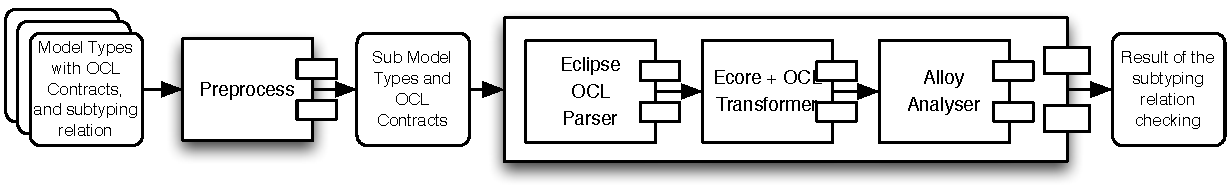
\includegraphics[width=5.3in]{fig/ToolSupport.pdf}
\caption{Contract Matching Checking Tool Overview}
\label{fig:toolsupport}
\end{figure}

The contract matching approach described in the previous subsection has been implemented in a prototype tool.
Figure \ref{fig:toolsupport} shows an overview of the prototype tool.
It consists of an OCL parser, an Ecore\footnote{Ecore is an implementation aligned with MOF included in the Eclipse Modeling Framework \cite{steinberg2008emf}.}/OCL transformer and the use of the Alloy Analyzer.
The Ecore/OCL transformer is developed using Kermeta \cite{muller2005weaving}, an aspect-oriented metamodeling tool. 
The inputs of the prototype are (1) an Ecore file that specifies two model types, and (2) a textual OCL file that specifies the contracts from each model type. 
The model types and contracts are automatically transformed to an Alloy model consisting of signatures and predicates.

The prototype provides several interfaces to check contract matching.
For example, {\em matchInv(inv1: Constraint, inv2: Constraint)} is used to check whether $inv1$ matches $inv2$.
In addition, {\em matchInvs(cls1: Class, cls2: Class)} can be used to check whether the invariants defined in $cls1$ and the invariants defined in $cls2$ match. 
%A relation query is transformed to an Alloy assertion that is added to the generated Alloy model.   

%The prototype then uses the APIs provided by the Alloy Analyzer to pass the Alloy model to the Alloy SAT solver.
%The result returned by the Alloy SAT solver is interpreted by the prototype to get feedback on the relation between two contracts. This relation is then used to check a declared subtyping relation between two model types. 

\subsection{Case Study}\label{casestudy}

In this section we illustrate how to use our approach to define model types and subtyping relations between them to ensure a safe reuse of model transformations.

\subsubsection{A Simple Case Study of Structural Substitutability}

\begin{figure}[!t]
\centering
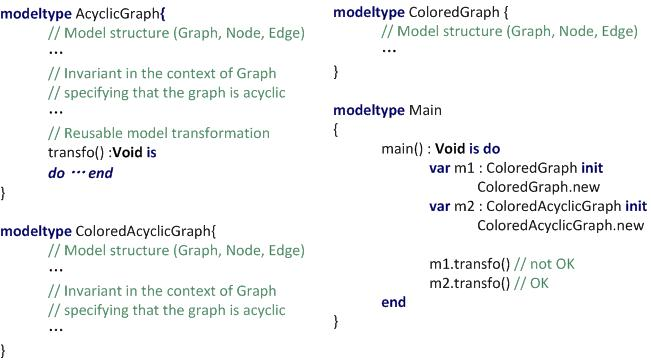
\includegraphics[width=4.8in]{fig/CaseStudy1.jpg}
\caption{A Simple Example of Structural Substitutability in Kermeta}
\label{fig:casestudy1}
\end{figure}

Let us reconsider the scheduling example described in Section \ref{structuralexample}.
A model transformation performs a static scheduling on an acyclic dependence graph.
The model transformation needs a metamodel for ``Acyclic Graph'' (due to space limitation, the metamodel is not shown in the paper).  
The model type $AcyclicGraph$ (see Figure \ref{fig:casestudy1}) shows a simple example of model type definition for the dependency graph used in the example. 
Its definition consists of metaclasses that specify a graph structure, an invariant that specifies the acyclicity property, and a model transformation that takes as input an acyclic graph.

Suppose that in another context a colored graph is used as an intermediate representation and it extends the concept of nodes by introducing additional information. 
To reuse the transformation defined in $AcyclicGraph$, a colored graph must be a subtype of $AcyclicGraph$. 
The model type $ColoredAcyclicGraph$ ensues the subtyping relation by adding an acyclicity invariant in its definition. However, the model type $ColoredGraph$ does not specify any invariants. 
A compilation error will thus show that the $transfo$ operation cannot take as input an instance of $ColoredGraph$ because $ColoredGraph$ is not a subtype of $AcyclicGraph$. 


\subsubsection{A Simple Case Study of Behavioral Substitutability}

\begin{figure}[!t]
\centering
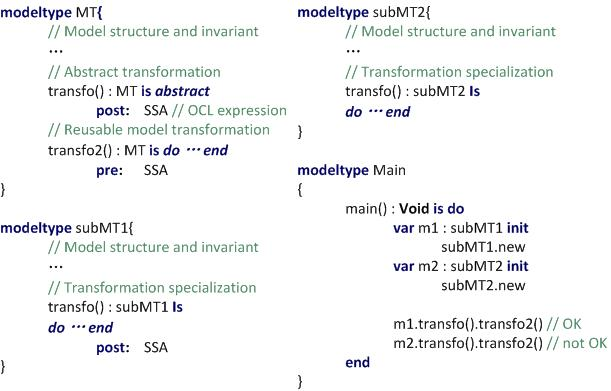
\includegraphics[width=4.8in]{fig/CaseStudy2.jpg}
\caption{A Simple Example of Behavioral Substitutability in Kermeta}
\label{fig:casestudy2}
\end{figure}

In the optimizing compiler community, the daily task for software engineers is to design compilation chains in the right partial order, that is, scheduling the various passes (i.e., optimization, translation, code generation, analysis, etc.).
Designing compilation chains would benefit from behavioral substitutability by opening the way to describe ``abstract'' compilation chains, capitalizing a given knowledge in terms of constraints (pre-/post-conditions) to schedule a set of passes for a given purpose, where each pass would be then implemented in various ways, but conforming to the pre-/post-conditions defined in the abstract compilation chain.    

Figure \ref{fig:casestudy2} shows a simple example of model types used for the compilation chain. 
Suppose that the abstract model transformation $\mathit{transfo}$ defined in $MT$ is used for optimization purpose and define a post condition stating that the model must conform to the Static Single Assignment (SSA) form. $MT$ also contains $\mathit{transfo2}$ as the next pass of the compilation chain and states as precondition that the model must conform to the SSA form. 
The two model types $subMT1$ and $subMT2$ implement the model transformation $\mathit{transfo}$ but only $subMT1$ ensures as postcondition the SSA form. While $subMT2$ is not in this case a sub model type to $MT$, a compilation error for $m2.$$\mathit{transfo}().$$\mathit{transfo}2()$ will be returned. This shows that the model returned by $\mathit{transfo}$ in $subMT2$ (typed by $subMT2$) is not of type $MT$, and can not reuse $\mathit{transfo2}$.

\section{Discussion}\label{discussion}

In this section we discuss limitations of our work, and its scope of application. 
We first discuss the supported contracts in the subtyping relation of model typing (Section \ref{sec:discussion:oclcontracts}), and the corresponding model substitutability provided by our approach (Section \ref{sec:discussion:substitutability}).

\subsection{On the Support of Contracts in Model Typing}
\label{sec:discussion:oclcontracts}
%% ==> FIRST PART OF THE TITLE

%Contracts > 1st order logic > OCL > subset supported by the translation to Alloy 
%But... we know that!

% IN OUR PAPER, we consider CONTRACTS in addition to object oriented metamodels
In this paper we consider contracts in addition to the object oriented structure described in a metamodel. The object-oriented structure is usually defined using Ecore, an implementation aligned with OMG MOF. Contracts can then be invariants expressed in the context of the concepts (i.e., classes) defined in the MOF metamodel, and pre-/post-conditions expressed in the context of operations specified in concepts. While invariants restrict the structure of conforming models and their possible structural substitutability, pre- and post-conditions specify the behavior of the conforming models (i.e. manipulation by model operations) and their possible behavioral substitutability.

% IN OUR APPROACH, we consider OCL CONTRACTS
In our approach, we assume that the first order logic is used to express contracts in metamodels, and we have chosen OCL to express them. We rely on the provided binding between MOF and OCL as defined by OMG to link OCL expressions to a given MOF metamodel.

% IN OUR TOOL, we consider the SUBSET OF THE OCL CONTRACTS supported by the translation to alloy
To test the feasibility of our approach, we implemented a prototype tool that is integrated into the Kermeta workbench. The tool checks OCL-based contract-aware subtyping relations between model types. While the substitutability related to the MOF structure is computed directly using Kermeta, the one related to the contracts is computed using Alloy through a translation from OCL expressions to Alloy specifications, and then an analysis of the output provided by the Alloy Analyzer. The tool only provides support for translating a subset of OCL to Alloy.

% IN OUR TOOL -> SUPPORTED part
Most of the OCL operators have corresponding Alloy constructs. For example, OCL operator $forAll$ corresponds to Alloy construct $all$, $exists$ corresponds to $some$, $includes$ corresponds to $in$, $excludes$ corresponds to $!in$, $sum$ corresponds to $sum$, and $closure$ corresponds to $*$. OCL contracts that involves such operators can be directly transformed into Alloy specifications.

% IN OUR TOOL -> NOT (or PARTIALLY) SUPPORTED part
However, as pointed out by Anastasakis et al. \cite{anastasakis2010challenges}, the translation from OCL to Alloy is not seamless. There are some OCL operators that do not have corresponding Alloy constructs, and thus OCL contracts including such operators cannot be easily transformed into Alloy specifications.  
%
Some of them can be partially supported by the tool using the Alloy libraries. For instance, OCL operators like $select$ and $collect$ are translated by the tool described in the paper using Alloy functions that implement their semantics. Consequently, the operator $iterate$ is partially supported by the transformation tool. The tool provides support for OCL contracts including $iterate$ expressions that can be rewritten as $forall$ with $select/collect$ operators. However, the tool cannot be used to deal with $iterate$ expressions that involve arithmetic accumulation since Alloy is a purely declarative language that does not provide support for imperative accumulators. Finally, the translation cannot deal with OCL casting operators like $oclAsType$ since Alloy has a very simple type system that has little support for type casting.

%SMT solvers address this problem. At some point we should look at tools such as Z3 from Microsoft in addition to Alloy.

\subsection{On the Support of Modeling Language Substitutability}
\label{sec:discussion:substitutability}
%% ==> SECOND PART OF THE TITLE

%% we support CONTRACTS FOR SUBSTITUTABILITY...
The research work described in the paper builds upon our previous work in \cite{ecmfa12}, and paves the way for reasoning about the subtyping relation between two model types that include contracts. 
Specifically it can be used to reason about the contract-aware subtyping relation that involves structural subtyping (including not only MOF-based Object-Oriented structure but also OCL-based first order invariants) and behavioral subtyping (including a behavioral semantics in an axiomatic way using pre-/post-conditions on operations).

%% ... in a practical way IN KERMETA
%The Kermeta workbench we use to develop the tool described in the paper is a language workbench that allows modelers to design languages using dedicated meta-languages: Ecore (for the abstract syntax), OCL (for the static semantics, i.e. invariants in the abstract syntax + pre-/post-conditions on operations to provide an axiomatic semantics), and the Kermeta language (for the operational semantics). 
We implement our approach in a (Kermeta-based) tool included in the Kermeta language workbench to check advanced (i.e., including contracts) subtyping relations between modeling languages based on Ecore and OCL. These two meta-languages are supported by the Kermeta language workbench and are used for describing the abstract syntax and the static semantics respectively. 

%% => scope of STRUCTURAL substitutability
This approach and its corresponding implementation addresses the need illustrated by the motivating examples from the high-performance embedded system community used throughout the paper. The scope of the structural substitutability we offer is bounded by OCL and its translation to Alloy, and its applicability is well founded, e.g., in model transformation reuse in model-driven development \cite{ecmfa12}.

%% => scope of BEHAVIORAL substitutability
The actual scope of behavioral substitutability is more difficult to define. The difficulty is twofold: while we support the motivating examples described in the paper, complex situations of OCL based typing could be considered, such as type propagation in model transformation chains. Such challenges will be addressed in future work. % and will be detailed in the concluding remarks of the paper. 
Moreover, the scope itself of behavioral substitutability is more difficult to delimit. 
%While it leverages an axiomatic semantics to specify behavioral properties that must be ensured for a safe model transformation reuse, such properties must be reflected into structural information of the input and output models (conforming to the same metamodel) to be expressed. Beyond that, other advanced application of behavioral substitutability should be explored in the future, and the tool-supported approach we provide in this paper is a well-fitted contribution for that. 



\section{Related Work}\label{relatedwork}

The technical contribution of this paper is the integration of contract matching in the subtyping relation of model typing to enhance the substitutability supported between modeling languages. As discuss in the previous section, we rely for that on the most established translation to Alloy. Then, the work related to our contribution discussed in this paper is the applicability of the substitutability as illustrated in the motivating examples, namely on model transformation reuse.

Substitutability is supported through subtyping in object-oriented languages, including the support of contracts (\emph{e.g.}, Eiffel \cite{Meyer98a}). However, object subtyping does not handle type group specialization (\ie the possibility to specialize relations between several objects and thus groups of types)\footnote{We refer the reader interested in the type group specialization problem to the Ernst's paper~\cite{Ernst01}.}. Such type group specialization have been explored by K\"{u}hne in the context of MDE~\cite{Kuhne12}. K\"{u}hne defines three model specialization relations (specification import, conceptual containment and subtyping) implying different level of compatibility. We are only interested here in the third one, subtyping, which requires an \emph{uncompromised mutator forward-compatibility}, \eg substitutability, between instances of model types.

Several approaches have been proposed during the last decade for model transformation reuse. Strict substitutability relation, such as the first version of model type matching presented in \cite{Steel07}, offers the possibility to reuse model transformation through isomorphic metamodels, i.e., metamodels with MOF-based equivalent structures. Such possibility was first proposed in~\cite{Varro04} where the authors introduce \emph{variable entities} in patterns for declarative transformation rules. These entities express only the needed concepts (\emph{e.g.}, types, attributes, etc.) to apply the rule, allowing any tokens with these concepts to match the pattern and thus to be processed by the rule. Latter, Cuccuru \emph{et al.} introduced the notion of semantic variation points in metamodels~\cite{Cuccuru07}. Variation points are specified through abstract classes, defining a \emph{template}, and metamodels can fix these variation points by binding them to classes extending the abstract classes. Patterns containing \emph{variable entities} and \emph{templates} can be seen as kinds of model types where the variability has to be explicitly expressed and thus anticipated.
%
Sanchez Cuadrado \emph{et al.} propose in~\cite{Sanchez08} a notion of substitutability based on model typing and model type matching, but rather to use an automatic algorithm to check the matching between two model types, they propose a DSL that allows users to declare the matching by hand.
%
Finally, De Lara \emph{et al.} present in~\cite{deLara10} the \emph{concept} mechanism, along with \emph{model templates} and \emph{mixin layers} leveraged from generic programming to MDE. \emph{Concepts} are really close to model types as they define the requirements that a metamodel must fulfill for its models to be processed by a transformation, under the form of a set of classes. The authors also propose a DSL to bind a metamodel to a \emph{concept} and a mechanism to generate a specific transformation from the binding and the generic transformation defined on the \emph{concept}.

%Further, adaptation allows the reuse of model transformations between metamodels in spite of structural heterogeneities. Two approaches have been considered. The first one is to adapt models conforming to a metamodel $M$ into models conforming to metamodel $M'$ on which is defined the transformation of interest. The second one is to adapt the transformation defined on $M'$ to obtain a valid transformation on $M$.
%
%In~\cite{Kerboeuf11} Kerboeuf \emph{et al.} present an adaptation DSL named \emph{Modif} which handles deletion of elements from a model (which conforms to a metamodel $M$) to make it substitutable to an instance of the metamodel $M'$. For this, a trace of the adaptation is kept to be able to go back from the result of the transformation (conforming to $M'$) to the corresponding instance of $M$. For example, in~\cite{Sanchez11} and~\cite{Wimmer11} the binding mechanism presented for \emph{concepts} in~\cite{deLara10} is extended to go further than strict structural mapping by allowing renaming, mapping of several elements from a metamodel to a single element from a \emph{concept} and navigation and filtering using OCL expression. These adaptations are possible through an hybrid approach which mixes model adaptation and transformation adaptation. This approach allows the same kind of adaptations than the injection of Kermeta aspects such as presented in \cite{Sen10}. However, the adaptations are automatically generated, either under the form of helpers or directly in the specific transformation which is generated from the generic transformation and the binding, while Kermeta aspects are added by hand.

%If these approaches make it possible to go further than reuse between isomorphic metamodels, there remain some heterogeneities which can not be handle automatically for now, such as different representation of the same information (\emph{e.g.}, a reference and a class representing the same concept). Moreover, none has, to our knowledge, addressed the problems of contracts and are limited to object-oriented structures. The tool-supported approach that we propose paves the way of both complex structural properties and behavioral properties for safe model transformation reuse through a formal unified theory of model typing. 

%% In the context of model transformation chains, it is often really hard to write the various passes in the right way. ... Our approach allow us to write the flow in an abstract way through pre and post, and then to implement the abstract model types: TO BE ADDED....

In the context of model transformation chains, existing approaches deal with explicit relationships between model transformations. Vanhooff et al. \cite{vanhooff2007uniti} proposed a domain specific language to model and execute a transformation chain. 
%
Aranega et al. \cite{aranega2012using} used feature models to classify model transformations involved a transformation chain and specified the constraints between them. The user thus can design a new transformation chain by reusing the classified transformations.   
%
Yie et al. \cite{yie2012realizing} advocated the use of several independently developed model transformation chains to convert a high-level model into a low-level model. The interoperability among model transformation chains is achieved by deriving correspondence relationships between the final models generated by each model transformation chain. 

Unlike the above approaches, contract-aware model subtyping offers a unified and formal type theory to facilitate the safe reuse of model transformations involved in a transformation chain. It follows a declarative fashion to specify a model transformation chain in an abstract way using pre-/post-conditions on abstract model types. This promotes then the reuse of various implementations that match the conditions for a safe execution of the model transformation chain.


\begin{comment}
\subsection{Model Transformation Reuse}

Iacob et al. \cite{iacob2008reusable} described a design pattern based approach for model transformation reuse.
The approach focuses on identifying and documenting reusable model transformation patterns.
Their approach, however, can only provide support for reusing part of transformation rules that are captured by the transformation pattern.

Cuadrado et al. \cite{Sanchez08} used factorization and composition of transformation definitions to enhance the reusability of model transformation.
The approach factorizes common parts of transformation definitions that are intended for reuse via composition and adaptation. 
Their approach, however, requires the input metamodel and the output metamodel of a transformation to have common model elements.

Cuadrado et al. \cite{Sanchez11} proposed a generic approach for model transformation reuse.
The approach uses templates to specify transformation rules in the context of a generic metamodel.
The templates are later bound to specific metamodels that conform to the generic metamodel.
The conforming relation between the generic metamodel and specific metamodels described in \cite{Sanchez11} is similar to one of the model subtyping relations (i.e., total non-isomorphic subtyping relation, cf. Def. 13 of \cite{ecmfa12}) described in our previous work. 

Sen et al. \cite{Sen10} presented an approach to reusing model transformations across several similar metamodels. 
The approach uses the slicing technique to obtain parts of a metamodel that are involved in a specific transformation.
The sliced metamodel is used as a model type, and the specific transformation can be reused in the metamodels that conform to the model type. 
Their approach builds upon a very simple model type system, and thus cannot provide support for contracts reuse.

Lara and Guerra \cite{deLara11} introduced $concepts$ (supertype) to capture structural and behavioral requirements for models and metamodels.
Model management operations (e.g., transformation operations) that defined over $concepts$ can be reused to any metamodels conforming to $concepts$.
Unlike the model subtyping relation, the conforming relation described in \cite{deLara11} is determined by an explicit binding between $concepts$ (supertype) and metamodels (subtypes).

\subsection{Model Transformation Chain}

Vanhooff et al. \cite{vanhooff2007uniti} proposed a domain specific language to model and execute a transformation chain.
Their work described in \cite{von2008constructing} focuses on generating diagrams to visualize the traceability information among intermediate and final models produced from the transformation chain execution.

Aranega et al. \cite{aranega2012using} used feature models to classify model transformations involved a transformation chain. The user thus can design a new transformation chain by reusing the classified transformations.   

Yie et al. \cite{yie2012realizing} advocated the use of several independently developed model transformation chains to convert a high-level model into a low-level model. The interoperability among model transformation chains is achieved by deriving correspondence relationships between the final models generated by each model transformation chain. 

Unlike the above approaches, contract-aware model subtyping relation offers a unified type theory to facilitate the reuse of model transformations involved in a transformation chain. 
\end{comment}

\section{Conclusion and Perspective}\label{conclusion}

%In this paper we extended model typing by taking into account contract-aware substitutability where contracts are defined in terms of invariants and pre-/postconditions expressed using OCL. 
We propose in this paper a model typing theory where model types include contracts. 
This includes a formally defined subtyping relation between model types, and a tool-supported approach supporting a safe contract-aware substitutability of models conforming to metamodels including contracts. This ensures a safe reuse of model transformations expressed on metamodels including contracts.

Contracts are defined in terms of invariants and pre-/post-conditions expressed using OCL on MOF-based metamodels. 
The invariants are added on the classes of a metamodel to specify additional structural properties of the metamodel, and pre-/post-conditions are added on the operations of classes to specify model transformations. 
%
Consequently, the support of invariants in the subtyping relation ensures a safe reuse of model transformations where OCL contracts are needed to precisely specify the structure on which the model transformation can be applied. The support of pre-/post-conditions paves the way for behavioral substitutability to safely reuse model transformations where OCL contracts are needed to precisely specify the applicability of the model transformation.

The subtyping relation is based on a matching relation between two MOF classes that include OCL contracts, and is checked thanks to a technique based on Alloy. The actual scope of the provided contract-aware substitutability is mainly determined by the OCL-to-Alloy translation.

%
%We also provide a research prototype to rigorously reason about the subtyping relation between two model types with contracts.
%The current version of prototype takes as input Ecore model types and OCL contracts.  
We are currently extending the prototype by providing support for model types and contracts expressed using the Kermeta language workbench.  We also explore how we can extend the approach by using SMT solvers at back-end to analyze the OCL contracts that include more complex arithmetic calculation.

\subsubsection*{Acknowledgment}
%
% For French admin issues:
This work was supported by the National Science Foundation grant (CCF-1018711), the ANR INS Project GEMOC (ANR-12-INSE-0011), and the CNRS PICS Project MBSAR.

\bibliographystyle{splncs}
%\bibliographystyle{unsrt}
\bibliography{ecmfa12-contractmatching}

%\newpage
%\appendix
%\input{isomorphism.tex} 


\end{document}
% vi:spell spelllang=en:
